%\documentclass[tikz,border=3pt,convert={density=600,outext=.png}]{standalone}
\documentclass[tikz,border=3pt]{standalone}

\usepackage[utf8]{inputenc} % utf8 encoding
\usepackage{amsmath,amsfonts} % nice math symbols

\usepackage{tikz}
\usetikzlibrary{arrows,shapes}

\begin{document}
	
	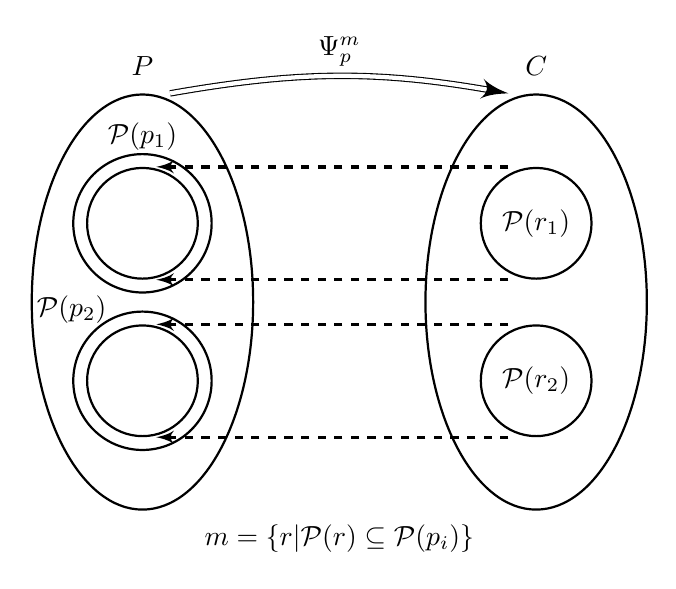
\begin{tikzpicture}
		\tikzstyle{ell}=[draw, thick, align=center]
		
		\node[ell, ellipse, minimum height = 150, minimum width = 80] (p) at (0,0){};
		\node at (0,3) {$P$};
		\node[ell, circle, minimum size = 50] at (0, 1) {};
		\node[ell, circle, minimum size = 40] (p_1) at (0, 1) {};
		
		\node[ell, circle, minimum size = 50] at (0, -1) {};
		\node[ell, circle, minimum size = 40] (p_2) at (0, -1) {};
		
		\node[ell, ellipse, minimum height = 150, minimum width = 80] (c) at (5,0) {};
		\node at (5,3) {$C$};
		\node[ell, circle, minimum size = 40] (c_1) at (5, 1) {$\mathcal{P}(r_1)$};
		\node[ell, circle, minimum size = 40] (c_2) at (5, -1) {$\mathcal{P}(r_2)$};
		
		\node at (0,2.1) {$\mathcal{P}(p_1)$};
		\node at (-0.9,-0.1) {$\mathcal{P}(p_2)$};
		
		\draw[-latex', very thick, dashed] ([xshift=-10]c_1.north) -- ([xshift=5]p_1.north);
		\draw[-latex', very thick, dashed] ([xshift=-10]c_1.south) -- ([xshift=5]p_1.south);
		\draw[-latex', very thick, dashed] ([xshift=-10]c_2.north) -- ([xshift=5]p_2.north);
		\draw[-latex', very thick, dashed] ([xshift=-10]c_2.south) -- ([xshift=5]p_2.south);
		\draw[-latex',double equal sign distance] ([xshift=10]p.north) to[bend right=-10] node[above]{$\Psi_p^m$} ([xshift=-10]c.north);
		
		\node at (2.5, -3) {$m=\{r|\mathcal{P}(r)\subseteq\mathcal{P}(p_i)\}$};
	\end{tikzpicture}

	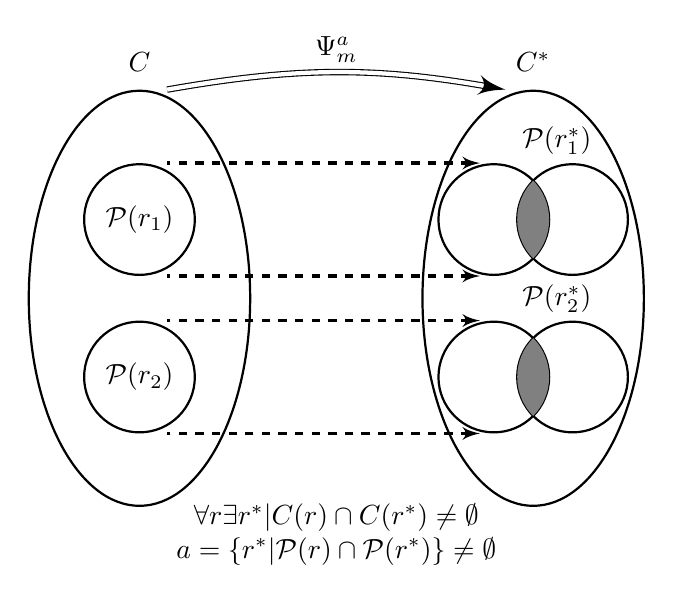
\begin{tikzpicture}
		\tikzstyle{ell}=[draw, thick, align=center]
		
		\node[ell, ellipse, minimum height = 150, minimum width = 80] (p) at (0,0){};
		\node at (0,3) {$C$};
		\node[ell, circle, minimum size = 40] (p_1) at (0, 1) {$\mathcal{P}(r_1)$};
		
		\node[ell, circle, minimum size = 40] (p_2) at (0, -1) {$\mathcal{P}(r_2)$};
		
		\node[ell, ellipse, minimum height = 150, minimum width = 80] (c) at (5,0) {};
		\node at (5,3) {$C^*$};
		\node[ell, circle, minimum size = 40] (c_1) at (4.5, 1) {};
		\node[ell, circle, minimum size = 40] (d_1) at (5.5, 1) {};
		\begin{scope}
			\clip (4.5,1) circle (20pt);
			\fill[gray] (5.5,1) circle (20pt);
		\end{scope}
		\node[ell, circle, minimum size = 40] (c_2) at (4.5, -1) {};
		\node[ell, circle, minimum size = 40] (d_2) at (5.5, -1) {};
		\begin{scope}
			\clip (4.5,-1) circle (20pt);
			\fill[gray] (5.5,-1) circle (20pt);
		\end{scope}
		
		\node at (5.3,2) {$\mathcal{P}(r_1^*)$};
		\node at (5.3,0) {$\mathcal{P}(r_2^*)$};
		
		\draw[latex'-, very thick, dashed] ([xshift=-5]c_1.north) -- ([xshift=10]p_1.north);
		\draw[latex'-, very thick, dashed] ([xshift=-5]c_1.south) -- ([xshift=10]p_1.south);
		\draw[latex'-, very thick, dashed] ([xshift=-5]c_2.north) -- ([xshift=10]p_2.north);
		\draw[latex'-, very thick, dashed] ([xshift=-5]c_2.south) -- ([xshift=10]p_2.south);
		\draw[-latex',double equal sign distance] ([xshift=10]p.north) to[bend right=-10] node[above]{$\Psi_m^a$} ([xshift=-10]c.north);
		
		\node[align=center] at (2.5, -3) {$\forall r\exists r^* | C(r)\cap C(r^*)\not = \emptyset$\\
			$a=\{r^*|\mathcal{P}(r)\cap\mathcal{P}(r^*)\}\not = \emptyset$};
	\end{tikzpicture}
	
	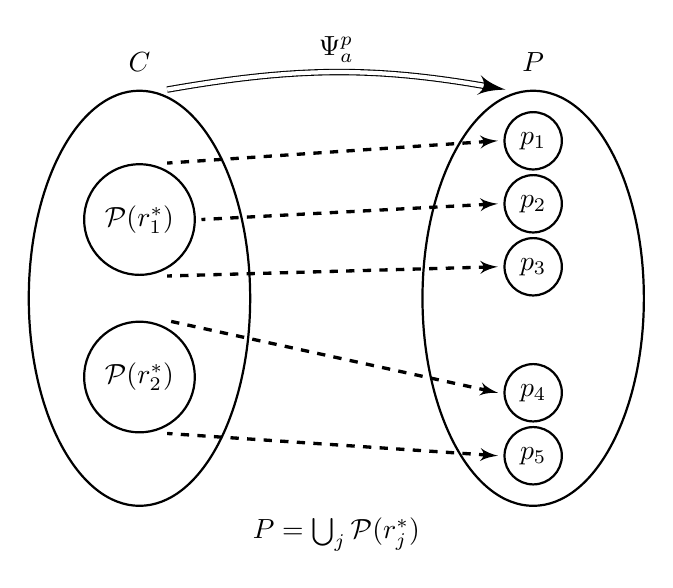
\begin{tikzpicture}
		\tikzstyle{ell}=[draw, thick, align=center]
		
		\node[ell, ellipse, minimum height = 150, minimum width = 80] (p) at (0,0){};
		\node at (0,3) {$C$};
		\node[ell, circle, minimum size = 40] (p_1) at (0, 1) {$\mathcal{P}(r_1^*)$};
		
		\node[ell, circle, minimum size = 40] (p_2) at (0, -1) {$\mathcal{P}(r_2^*)$};
		
		\node[ell, ellipse, minimum height = 150, minimum width = 80] (c) at (5,0) {};
		\node at (5,3) {$P$};
		\node[ell, circle, minimum size = 10] (c_1) at (5, 2) {$p_1$};
		\node[ell, circle, minimum size = 10] (c_2) at (5, 1.2) {$p_2$};
		\node[ell, circle, minimum size = 10] (c_3) at (5, 0.4) {$p_3$};
		\node[ell, circle, minimum size = 10] (c_4) at (5, -1.2) {$p_4$};
		\node[ell, circle, minimum size = 10] (c_5) at (5, -2) {$p_5$};
		
		
		\draw[latex'-, very thick, dashed] ([xshift=-2]c_1.west) -- ([xshift=10]p_1.north);
		\draw[latex'-, very thick, dashed] ([xshift=-2]c_2.west) -- ([xshift=2]p_1.east);
		\draw[latex'-, very thick, dashed] ([xshift=-2]c_3.west) -- ([xshift=10]p_1.south);
		\draw[latex'-, very thick, dashed] ([xshift=-2]c_4.west) -- ([xshift=10]p_2.north);
		\draw[latex'-, very thick, dashed] ([xshift=-2]c_5.west) -- ([xshift=10]p_2.south);
		\draw[-latex',double equal sign distance] ([xshift=10]p.north) to[bend right=-10] node[above]{$\Psi_a^p$} ([xshift=-10]c.north);
		
		\node at (2.5, -3) {$P=\bigcup_j\mathcal{P}(r_j^*)$};
	\end{tikzpicture}

\end{document}